\chapter{Implementacja}
\label{cha:implementacja}

Ze względu na charakter aplikacji, która składa się z autonomicznych elementów, znaczna część implementacji poszczególnych serwisów mogła odbywać się niezależnie od innych. Tworzone funkcjonalności testowane były przy pomocy narzędzia Postman, za pomocą którego można wysyłać dowolnie skonfigurowane zapytania HTTP na konkretne adresy URI. Kolejne, gotowe usługi były następnie integrowane w sytemie.

%---------------------------------------------------------------------------

\section{Metodyka pracy}
Projekt powstawał iteracyjnie. To znaczy, że podczas pracy zaczynano od małych celów i po ich realizacji - stawiano trochę większe, udoskonalano obecny wówczas stan i przechodzono do kolejnego, bardziej zaawansowanego kroku. W ten sposób, możliwe było dokładne kontrolowanie rozwoju systemu, jego testowanie i w razie problemów, szybka analiza i znalezienie ich przyczyny. 

\subsection{Version Control System}
\textbf{VCS} - postęp prac śledzony był za pomocą systemu kontroli wersji.
Pozwala on dokumentować wszystkie, kolejne zmiany, które mają miejsce w odniesieniu do kodu. Dzięki temu wygodniejsze są również potencjalne eksperymenty, ponieważ w każdym momencie, możliwy jest powrót do dowolnego, poprzedniego stanu implementowanych funkcjonalności.\cite{vcs}\\
W projekcie korzystano z hostingu na platformie GitHub.

\subsection{Organizacja zadań}
\textbf{Kanban} to metodologia, która może być użyta jako narzędzie do zarządania projektem podczas produkcji oprogramowania. Oryginalnie wymyślona w celu optymalizacji produkcji w Japońskiej firmie Toyota. Jej implementacja w procesie rozwijania systemów informatycznych znacząco wzrasta ze względu na przewagę nad tradycyjnymi metodami objawiącej się elastycznością, wydajnością i zwiększoną produktywnością. Sama nazwa oznacza w wolnym tłumaczeniu ``spis widoczny``.\cite{kanban}\\ Głównym elementem jest utworzenie torów, oznaczających poszczególne etapy w których znajdują się obecnie zadania. W momencie zmiany stanu, dany element jest przemieszczany do nastepnej w kolejności kolumny.\\
Korzystając z faktu, że w serwisie Github możliwe jest utworzenie takiej kanbanowej tablicy, zdecydowano się na użycie właśnie tej implementacji narzędzia. Poniżej zaprezentowano stan części planszy podczas rozwoju projektu.
\begin{figure}[H]
	\centering
	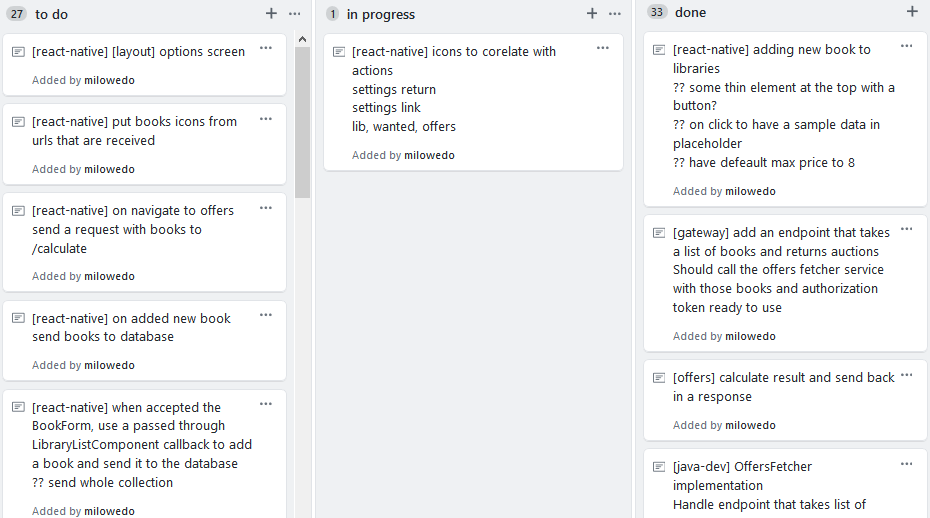
\includegraphics[width=\linewidth]{kanban.png}
	\caption{Kanbanowa tablica podzielona na 3 sektory}
\end{figure}

%---------------------------------------------------------------------------

\section{Wybór technologii}
Językami programowania, które maja największy udział w projekcie są Javascript(2.2, 2.3, 2.7) oraz Java(2.4). Za persystencję odpowiada chmurowa wersja bazy danych NoSQL(2.6.2) - MongoDB Cloud.\\

\subsection{Express}
\textbf{Auth Service} oraz \textbf{Gateway} to serwisy o podobnym stosie technologicznym. Obydwa powstały z pomocą Express js API - javascriptowego frameworku wspierającego implementację serwera obsługującego tworzenie i wystawianie REST API.
\begin{figure}[H]
	\centering
	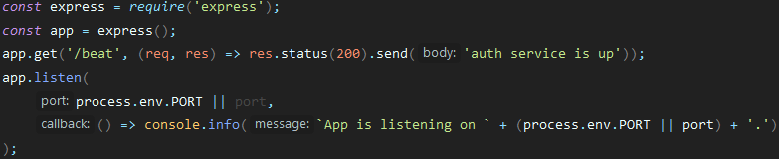
\includegraphics[width=\linewidth]{express_simple.png}
	\caption{Kod odpowiedzialny za wystawienie prostego API}
\end{figure}
Jak przedstawiono powyżej, aby stworzyć nasłuchujący na jednym punkcie końcowym serwer, wystarczy parę linijek kodu. Naturalnie, potrzeby wspomnianych serwisów są większe i potrzebują bardziej zaawansowanego podejścia niż przedstawiono na załączonej grafice.

\subsection{React Native}
\textbf{Aplikacja mobilna} jest napisana na platformie Expo, która jest zestawem narzędzi ułatwiającym prace w stworzonym przez Facebooka frameworku mobilnym - React Native. Został on wybrany, ponieważ jest sprawdzony(Facebook, Instagram, Skype), ciągle udoskonalany i prawdopodobnie nie przestanie być popularny w najbliższym czasie. Posiada on także pokaźną społeczność, co często okazuje się być nieocenionym podczas implementacji.\\
Ciekawym rozwiązaniem zaprezentowanym przez twórców są tak zwane Hooki, które pozwalają używać stanu w wykorzystanych w aplikacji komponentach funkcyjnych - lżejszych niż komponenty klasowe.\\

Przykładem zastosowania jest pobieranie książek (za pomocą funkcji fetchMyBooks()) z bazy danych - wywołanie to potrzebne jest jedynie raz, podczas pierwszego ładowania ekranu MyLibraryScreen. Nie jest pożądanym wysyłać zapytania za każdym razem, kiedy użytkownik powróci do tego samego punktu i tracić zasoby urządzenia - dane są już i tak obecne w pamięci podręcznej. 
\begin{figure}[H]
	\centering
	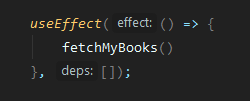
\includegraphics{hook.png}
	\caption{Zastosowanie hooka ``useEffect``}
\end{figure}
Hook \textbf{useEffect} przyjmuje dwa argumenty, pierwszy to funkcja, która ma się wykonać przy inicjalizacji komponentu oraz za każdym razem kiedy element tablicy z drugiego argumentu ulegnie zmianie.

%---------------------------------------------------------------------------

\section{Wielowątkowe tworzenie ofert}
\newpage
%---------------------------------------------------------------------------

\section{Autoryzacja użytkownika w Allegro API}

Do integracji serwisu z aplikacją potrzebne jest pozyskanie tokenu dostępowego. Allegro udostępnia tzw. ``ścieżkę device flow``, dzięki której cały proces odbywa się bez konieczności uwzględniania go w interfejsie graficznym. Poniżej zaprezentowany jest diagram prezentujący tę funkcjonalność.\\

\begin{figure}[H]
	\centering
	
\includegraphics[width=\linewidth]{device_flow.png}
	\caption{Autoryzacja użytkownika typu Device flow}
	\caption*{Źródło: {https://developer.allegro.pl/}}
\end{figure}

Podejście w tej pracy zakłada zarejestrowanie jednego, wspólnego dla całego systemu, konta funkcjonalnego za pomocą którego każde zapytanie będzie autentykowane. Stwarza to niestety jedno ograniczenie, a mianowicie, ze względu na obowiązujący główny limit nakładany na Client ID po przekroczeniu liczby 9000 zapytań na minutę, aplikacja zwróci status HTTP 429 i zostanie zabklokowana na kolejne 60 sekund.\\
W fazie inicjalizacyjnej autoryzacji uzyskane zostaną dwa unikalne tokeny: 
\begin{itemize}
	\item dostępowy - ważny przez 12h.
	\item odświeżający - ważny 6 miesięcy.
\end{itemize}
Zostaną one zachowanie w pamięci, a każde kolejne zapytanie, w przypadku wygaśnięcia tokenu dostępowego, spowoduje jego odnowienie.
\begin{figure}[H]
	\centering
	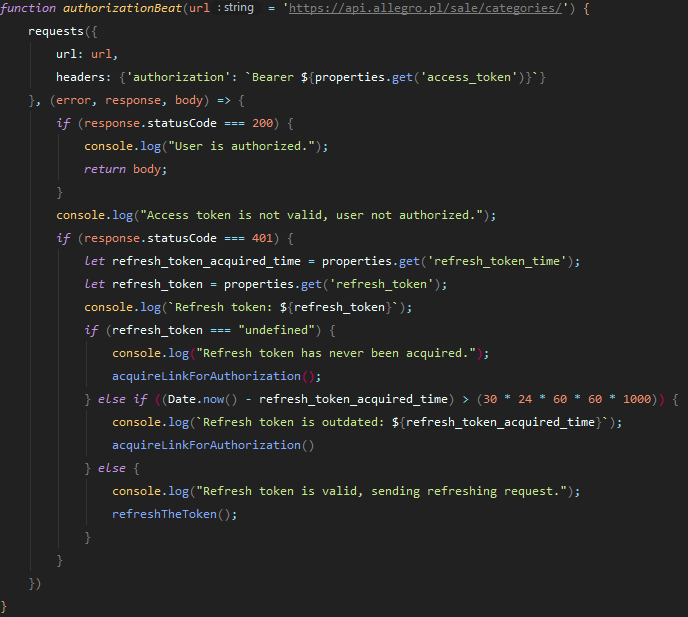
\includegraphics[width=\linewidth]{authorization.png}
	\caption{Kod odpowiedzialny za utrzymywanie ważnego tokena}
\end{figure}
Powyższy kod prezentuje przebieg akcji, które maja miejsce za każdym razem, kiedy otrzymywane jest zapytanie do OffersService(2.4). Na początku sprawdzane jest, czy token jest zwyczajnie aktualny, następnie, w przypadku, gdy nie jest, pobierany jest token odświeżający. W zależności od tego, czy jest on ważny, wygaśnięty, czy może w ogóle nigdy nie został uzyskany, odpowiednia logika zostaje uruchomiona.

%---------------------------------------------------------------------------

\section{MongoDB Cloud}
 
Modele przechowujące dane są zdefiniowane w klasach User.js i
oraz Book.js. Połączenie do bazy danych jest obsłużone przy pomocy bilbioteki ``mongoose``. Potrzebny jest jedynie tak zwany connection string, który uzyskany został poprzez zalogowanie się na stronie webowej serwisu hostującego cloud.mongodb.com i nawigację do zakładki Connect.\\
\begin{figure}[H]
	\centering
	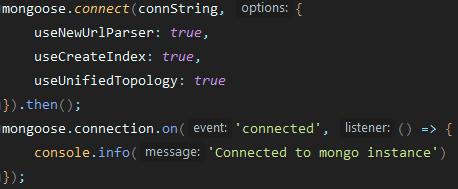
\includegraphics[width=\linewidth]{mongo.png}
	\caption{Połączenie do bazy danych MongoDB}
\end{figure}
W załączonej grafice widać rozpoczęcie połączenia z bazą danych. Ważnym elementem jest opcja \textbf{useCreateIndex}, dzięki której znajdujące się w serwisach Auth Service i Gateway, modele, otrzymają indeksy pod którymi znaleźć będzie można zapisane dokumenty. 

%---------------------------------------------------------------------------

\section{Wdrożenie}

Korzystanie ze stworzonych serwisów jest umożliwione poprzez wdrożenie ich na platformie chmurowej Heroku.
W ten sposób każda usługa posiada własne URI, na które wysyłane są zapytania w zależności od potrzeb.
Poszczególne aplikacje możnaby również uruchomić na pojedynczym komputerze, jednakże wymagałoby to sporej ilości zasobów, stąd zdecydowano się na rozwiązanie hostingowe.\\

Minimalne środowisko jakie jest wymagane aby uruchomić system to:
\begin{itemize}
	\item Node v10.13.0
	\item Java v11
	\item Maven v3.5
	\item Gradle v6.0
	\item Expo v3.11.1
\end{itemize}

Wdrożenie wymagało stworzenia aplikacji w sensie logicznym za pomocą lini komend Heroku CLI oraz wskazania adresu URI do stosownych repozytoriów Github, gdzie przetrzymywany jest kod.
W ten sposób w webowym interfejsie pod adresem dashboard.heroku.com znalazły się odnośniki reprezentujące trzy usługi : OffersFetcher, Auth Service oraz Gateway. Każda z nich ma zdefiniowaną odpowiednią konfigurację, dzięki której aplikacje mogą zostać uruchomione.
\begin{itemize}
	\item {OffersFetcher uruchamiany jest na platformie poleceniem \textit{web java -jar build/libs/*.jar}}
	\item {AuthService oraz Gateway - komendą \textit{npm start}}
\end{itemize}

Aby uruchomić lokalnie aplikację mobilną należy w folderze ją zawierającym wykonać polecenie \textit{expo r}.

%---------------------------------------------------------------------------